%%%%%%%%%%%%%%%%%%%%%%%%%%%%%%%%%%%%%%%%%%%%%%%%%%%%%%%
%%%%%%%%%%%%%%%%% INTRODUCTION %%%%%%%%%%%%%%%%%%%%%%%%
%%%%%%%%%%%%%%%%%%%%%%%%%%%%%%%%%%%%%%%%%%%%%%%%%%%%%%%

\chapter{Introduction}
\label{Introduction}

%\subsection{Background Kant}
%In Kant's Prolegomena %or maybe somewhere else
%he calles Euclidean geometry as a priori. 
%Euclidean geometry is based on the five axioms, the fivth being the paralell axiom \cite{Coxeter.1998}.
%When Kant is calling a piece of information a priori, this means, this information must be  true. But as the fifth axiom is not necessarily given in non-Euclidean geometry geometry, Euclidean geometry cannot be a priori. This opens a wide discussion on to what extend Kant's further conclusions are all invalid. 
% Kants opinions
% non euclidean geometry would falsify what of Kants opinion 
\section{Euclidean and non-Euclidean geometry} 
When we see something, we expect it to be also found in the physical world. We have learnt that when we see something, physical interaction confirms us that it is actually found there. If one had to explain  the geometry of what we see, they would say that it is most likely an identical depiction of the actual world. Thus as we interact with our world, as if it was a Euclidean space, we would also expect our visual space to be Euclidean space.

Euclidean space is something we are very familiar with. In two dimensions it simply is a plane. For example on a map of a town we can describe the position of a building using coordinates. If we were to choose two distances on the map with the same length, they would represent the same physical distance. %helpfull?
For all two points one would choose on such a map the shortest path between the two points is always a straight. Euclid had five postulates for his geometry, the latest of which was later on called the axiom of parallelism: "There is at least one line $q$ and at least one point $A$, not on $q$, such that no more than one line can be drawn through $A$ coplanar but not meeting $q$" \cite[p.~186]{Coxeter.1998}.

Non-Euclidean geometry is something we are more seldomly confronted with in our everyday lives. Gauss was the first to make non-Euclidean space applicable \cite{Parrochia.2018}. In such a space the shortest path between two points is not necessarily a straight. He called the shortest path between two points a geodesic. On our map the geodesic between any two points would be a straight, but in a non-Euclidean space it is different. Imagining the shortest path between London and Beijing, one can easily understand a geodesic. As our earth is not flat, the space we are in is non-Euclidean and the shortest path between the two cities is a geodesic. As the earth is roughly a sphere the geodesic is a circular arc.  %mathematical definition of a geodesic Gauß-Bonnet Theorem? %more general on non-euclidean space?
% schreibweise: \non-euclidean, oder non-Euclidean, eher letzteres
In non-Euclidean space, the just mentioned parallel postulate is not given \cite{Coxeter.1998}. For example, for the longitudes of our earth, being elliptic, the parallelism of these lines is not given as they all merge at the poles.
Later on, Riemann generalised Gauss' idea to manifolds of three or more dimensions \cite{Luneburg.1947}.

\section{Binocular vision}
One has to differentiate between the visual space and the physical space. Luneburg \citeyear{Luneburg.1947} defines the visual space as the visual sensation of our surrounding, not only including the colours and brightness of the objects of our surrounding, but also their localisation in a three-dimensional space. This space has got a geometry, which is then called the intrinsic geometry of the visual space. It needs to be differentiated from the extrinsic geometry, which describes the relationship between the visual space and its surrounding space \cite{Fernandez.2009}. This surrounding space is another way of measuring our environment by taking its physical measurements, for example by measuring the physical distance between two objects. Luneburg calls this the physical space. Scarcely surprising, they are mainly the same; after all, the visual space is a depiction of the physical space. But in some aspects they differ:

By having two eyes, two separate viewpoints are provided when perceiving the physical world. They allow binocular vision as two partially distinct images get transmitted, each by one eye. Our eyes have a common reference point called the egocenter, %was nützt diese Information?
located midway of the interocular axis, the axis between the two eyes \cite{DeValois.2000}. This allows the visual points of the two eyes to be mapped into one binocular space.
The result is then the one continuous image we call the seen image. 

There are visual points which are mapped onto the same position in both eyes. The horopter describes a group of such points. It is called horizontal horopter or frontal plane horopter, when examining the visual points on the horizontal plane in front of the eyes. One must distinguish between the theoretical and the empirical horopter. The theoretical horopter consists of the points furthest away from the eyes, which are mapped on corresponding positions on the retina. Hence the disparity of the two eyes at those points equals zero. Those are the points which are seen most easily \cite{DeValois.2000, Helmholtz.1867}. % ist dieser letzte satz hilfreich? berufts sich Helmholtz irgendwann auf diese Leichtigkeit?
They all align on a circular arc. The circle, they partly align on, is called a Vieth-Müller circle (see figure \ref{horopterLuneburg}).
\begin{figure}
    \centering
    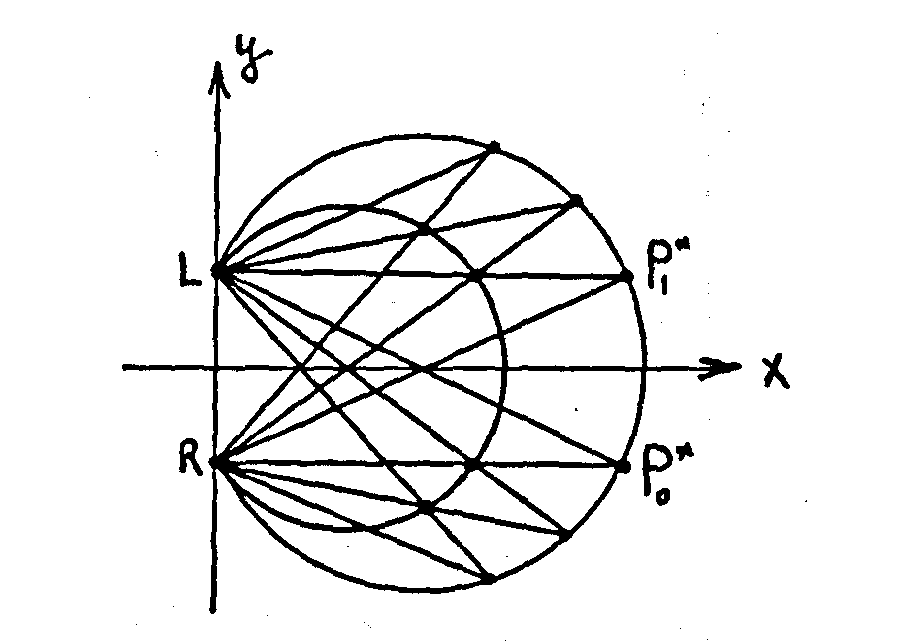
\includegraphics[width=7cm]{Images/Horopter from Luneburg 1950.png}%picture?
    \caption{The theoretical horopter. The points with zero disparity on both eyes are all found on the Vieth-Müller circle. L and R indicate left and right eye respectively. Taken from Luneburg (1950).} 
    \label{horopterLuneburg}
\end{figure}
The empirical horopter, on the other hand, is based on psychophysical observations, not on calculations, and differs from the Vieth-Müller circle. Its curvature can be steeper or flatter than the Vieth-Müller circle and it can be skewed \cite{DeValois.2000}.

The retinal image is only a two dimensional image lacking the third dimension, the depth dimension. Our brain reconstructs this dimension using different depth cues. 
Firstly, there is the stereopsis: the matching of the two retinal images allows depth perception, by using the binocular disparity \cite{Mallot.2000}. 
Other cues are lighting, hard shadow, at larger distances o\-pa\-ci\-ty, one object covering the other and the relative size of an object if the actual size is known. All these cues are based on experience \cite{Helmholtz.1867}.


\section{Luneburg's depth theory}
The basis for the depth theory is the geometrical analysis of binocular vision \cite{Helmholtz.1867, Luneburg.1947}. It is a purely mathematical analysis of binocular vision. Luneburg \citeyear{Luneburg.1950} himself said that his theory is no general theory of space perception as no psychological factors were included.
Von Helmholtz \citeyear{Helmholtz.1867} noticed that the visual space had a curvature. He placed 
three strings vertically next to each other on one plane. When looking at the strings, while the median plane of his face was cutting the middle string, the middle string appeared to be closer to him than the others. This effect increased by decreasing distance to the strings and even changed into the opposite at far distances (see figure \ref{empHoropterHelmholtz}). 
\begin{figure}
    \centering
    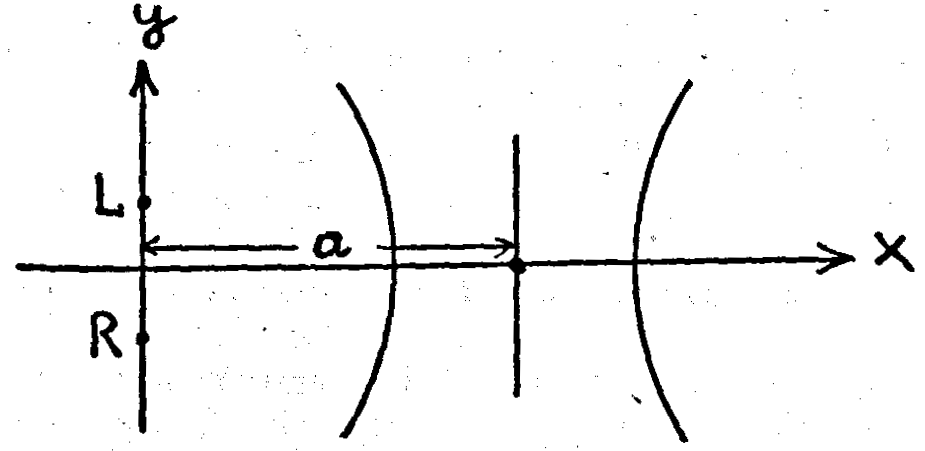
\includegraphics[width=7cm]{Images/HelmholtzEmpHoropter.png}%picture?
    \caption{Different empirical horopter curves for different fixations found by Helmholtz (1867). L and R indicate left and right eye respectively. Taken from Luneburg (1950).} %nicht optimal
    \label{empHoropterHelmholtz}
\end{figure}
%ref picture Luneburg
He concluded the visual space to be elliptic in near space. The extent of the effect, represented with $a$ in figure \ref{empHoropterHelmholtz}, was dependent on the person.
%to be elaborated

Luneburg went even further. He proposed the visual space to be of constant Gaussian curvature and derived a metric to translate from the physical space to the visual space. His hypothesis \citeyear{Luneburg.1947} was that the visual space is an integration of the information provided by the mathematical relation of the apparent size to the physical qualities of localisation and arbitrary parameters depending on the observer. %overkill
It depends on the physical position of the object, expressed in bipolar differentials, and depends on the localisation of the line element as one characterisation of the visual space. 
% ab hier möglicherweise streichen §§§§
The line element $ds$ can be represented by 
\begin{flalign}
ds^2 = dp^2 + \textnormal{sin}_K(\rho )^2 d\theta^2
\end{flalign}
where $\rho$ and $\theta$ are polar coordinates with $\rho$ denoting the perceived egocentric distance and $\theta$ denoting the perceived direction \cite{Heller.1997}. The function of $\textnormal{sin}_K(\rho)$ depends on $K$, i.e. if it is equal to zero, positive or negative. 
% bis hier §§§§
Luneburg assumes the value of $K$, denoting the Gaussian curvature, to be constant at any point in the visual space. The visual space is hyperbolic for $K > 0$, elliptic for $K < 0$ and Euclidean for $K = 0$.
He describes the curvature $K$ by 
\begin{flalign}
K = -e ^{-2\sigma \mu}
\end{flalign} where $\sigma$ and $\mu$ are constants. To determine these constants he leaves as a future research question \cite{Luneburg.1947}. He concludes the visual space to have a non-Euclidean geometry and conjectures it to be hyperbolic. He sees this confirmed  by observations of several authors, for example those of Blumenfeld in his alley experiments \cite{Blumenfeld.1913}, or those of von Helmholtz in his frontal horopter plane experiments \cite{Helmholtz.1867}.   

The necessity of the intrinsic curvature to be constant is controversial. %(Busemann, Freudenthal, Suppes) siehe Indow
Luneburg himself brought forth several arguments for a constant curvature \cite{Luneburg.1950}. If the metric space the distance function is defined on is homogeneous, the Riemannian space is of constant curvature. In empirical experiments a lack of absolute localisation was noticed and incorporating this principle into the psychometric distance function, this leads according to Luneburg to a homogeneous space. Secondly, as the appearance of the phy\-si\-cal object does not change when the object moves in the visual space, a constant curvature was assumed. This is related to the Helmoltz-Lie problem, %mäh
which discusses the conditions under which a physical object does not change size and shape when changing position \cite{Freudenthal.1965}. The solution is that physical space must be structured according to one of these geometries: $K = 0, K > 0, \textrm{or } K < 0$. Transferring this to the visual space, the visual space should be of constant curvature \cite{Indow.1991, Indow.1997}. On the other hand, some counter evidence to a constant curvature has already been found in experiments
\cite{Cuijpers.2001}.
%Gegenpositionen

One measure of the Gaussian curvature is given by the Gauss-Bonnet theorem.
Following this theorem, the total curvature of a polygon is measured by the angular excess \cite{wilson.2007}. For example, in a triangle in Euclidean space all angles add up to 180\textdegree{} \cite{Parrochia.2018}. 
The angular excess is hence the difference of the sum of the triangle's angles in non-Euclidean space to the angles' sum in Euclidean space. 
% absatz passt da eigentlich nicht rein. 
\section{Previous experiments}
Some have already tested Luneburg's hypothesis of the visual space being of constant curvature using different methods. The frontal plane horopter ex\-pe\-ri\-ment is based on the three-strings ex\-pe\-ri\-ment of Helmholtz \cite{Helmholtz.1867}. In the frontal plane horopter experiment subjects were asked to align several stimuli next to each other against a uniform background until they perceived them to be on a straight line. %discrimination of distant alley and parallel alley experiment?
In the alley experiment the subject also had to place stimuli on their eyes' horizontal plane, this time not parallel to their interocular axis but orthogonal \cite{Blumenfeld.1913}. At the far end two lights were fixed, the others had to be placed in two lines, so that the subject perceived them to be parallel. These experiments were usually conducted under non-natural conditions. They took place in the dark with only the lights being visible. The subjects' heads are placed on a headrest, hence only eye movement is possible. Thus in such an experiment only binocular disparity can be used as a depth cue. 

Zajaczkowska \citeyear{Zajackowska1956.} conducted both a frontal plane horopter experiment and alley experiments. He constructed three differerent alley experiments: the classic alleys, the intermediate alleys and the broad alleys, in which he varied increasingly the distance in between the furthest points. For his experiments he used Luneberg's formulas \cite{Luneburg.1950} to predict his results and to compare them with his own empirical data. The results of the frontal plane horopter experiment were close to the predictions. For subjects with a low absolute value of $K$ and good depth perception the measured and expected horopter differed less. The values of $\sigma$ (the higher, the better the depth perception) and $K$ were closest to the predicted for the broad alley experiment \cite{Zajackowska1956.}. %was ist mit mu passiert? 
As the subjects with good depth perception gave good support for Luneburg's hypothesis, he concluded on a non-Euclidean, hyperbolic visual space. 

Koenderink, van Doorn and Lappin \citeyear{Koenderink.2000} were the first to introduce the method of exocentric pointing to measure the geometry of the visual space and to test Luneburg's theory. They criticised the conditions of the pre\-ce\-ding experiments since those experiments having stimulus reduction to lights with no body movements allowed including head fixation (from now on called minimalistic experiments) did not measure up with our natural perception. They ascribed the preceding results to these constraints. Indeed, earlier experiments, which took place in an open field or a room with reference points, did not show constant curvature \cite{Cuijpers.2001, Battro.1976}.

That is why Koenderink et al. conducted their experiment in the field and allowed body movement. Only the eye height and the location the subjects were positioned at were constrained. Additionally, in contrary to Luneburg's theory, they did not assume the visual space to be of constant curvature, they only assumed the space to be Riemannian and isotropic \cite{Koenderink.2000}. They claimed to be able to describe the intrinsic curvature as a function of distance, i.e they expected the curvature of the intrinsic visual space to be dependent on the distance of the subject to the perceived objects. 

Exocentric pointing needs to be differentiated from normal pointing or aiming, as the object one is pointing with is at a different position than oneself. Hence the subject, the pointer and the target are all at three different positions, forming the three corners of a triangle. The task of the subjects was fairly simple, as to point with the pointer at the target. The pointer was rotatable on its y-axis by the subject via a remote controller. The construction of Koenderink et al. \citeyear{Koenderink.2000} for the pointer allowed good recognition of the pointer's orientation. The pointer consisted not only of an arrow for pointing, but the arrow was spiking a cube. This had the advantage that, additionally to the length of the arrow $(\alpha/\bar \alpha)$, the size's relation of the cube's faces $\lambda / (\lambda -1)$ indicated the pointer's orientation (see figure \ref{figSchematicPointer}). 
\begin{figure}
    \centering
    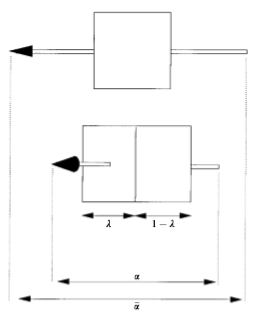
\includegraphics[width=6cm]{Images/PointerSkize.PNG}%picture?
    \caption{Schematic image of the pointer as it appears to the subject with relational sizes in the study of Koenderink et al. (2000).} %nicht optimal
    \label{figSchematicPointer}
\end{figure}

Their results showed a deviation from the veridical angle, hence also showed a curvature of the visual space. The deviation and therefore the intrinsic curvature depended on the distance of the subject to the target. Therefore Koenderink et al. \citeyear{Koenderink.2000} showed counter-evidence for Luneburg's hypothesis of constant intrinsic curvature. Their results suggested intrinsic visual space to be elliptic in near space and hyperbolic in far space.
%WHAT IS THIS STRANGE THING ABOUT -K AND STILL HYPERBOLIC SPACE?

\section{Aims of this study}%herleitung zum eigenen experiment
Our experiment is also going to try measuring the intrinsic geometry of the visual space by looking at possible deviations on the horizontal plane at eye height.
All preceding experimenters assumed the geodesics to be the best way to describe the curvature in their experiments. Even if a geodesic is a neat mathematical description of a curvature, it does not make the description necessarily more likely, especially if also the interference of other psychological factors is taken into account. Additionally, with the results of Koenderink et al. there are contradictory results concerning the constancy of the intrinsic visual space. Therefore our experiment is going to test Luneburg's hypothesis of a constant curvature again. It is going to use the method of exocentric pointing of Koenderink et al. \citeyear{Koenderink.2000}. 

Something that has not been considered enough so far is the influence of environmental cues on the depth perception. The surrounding may have a strong influence on the perceived depth; as described earlier, the environment provides many different depth cues. This may influence the deviation. In the minimalistic experiments this could have not been the case. That is why in our experiment there will be two conditions, one of which is a minimalistic experimental condition taking place in absolute darkness (in the following called dark condition), hence eliminating all environmental depth cues. The other one is conducted under natural illumination (in the following light condition). This comparison will allow us a first examination of that presumable environmental influence. 

%why virtual reality?
All preceding minimalistic experiments \cite{Zajackowska1956., Indow.1991} %(und co),
were conducted in lab rooms, which were darkened artificially. In many experiments today virtual reality glasses are used. They allow the stimuli to be more controlled. Using virtual reality glasses for the minimalistic experiments has many advantages. For example, absolute darkness can be guaranteed and all movement can be inhibited without a head rest. The subject may be absolute na\"{i}ve of the room structure and the targets' positions. Additionally, if using virtual reality is confirmed as a possible experimental set-up for exocentric pointing, this opens a wide range of possibilities: Stimuli, room or other cues can be tailored for the experiment without any restrictions \cite{Gaggioli.2001}. Those advantages need to be evaluated in relation to the drawbacks such as limited field of view or possible underestimation of distance \cite{Interrante.2008}.

\subsection{Hypotheses}
Parallel to this experiment another experiment took place with the same conditions, however not conducted in virtual reality, but in an actual lab room (in the following called real life experiment). We expect that our virtual reality experiment will provide similar results to the real life experiment.

Secondly, we expect the curvature not to be dependent on the side the pointer is standing at, i.e. we expect the curvature to be symmetrical in the dark condition, as in minimalistic experiments symmetry has already been shown \cite{Indow.1991}. In the light condition the symmetry could not be given as clearly as in the dark condition, as the surrounding environment not visible in the dark provides depth cues and thus may influence the perceived depth. These cues may be different when pointing into the opposite direction. 
If there is a difference between dark and light condition, the geodesics alone are possibly not sufficient to describe the intrinsic visual curvature. Then, interference of the structure of the room can be concluded.

Thirdly, our main hypothesis is that the deviation of the angle, i.e. the error the subjects are making, will depend on the angle of the pointer in relation to the target and the subject and will display no constant curvature. This angle is dependent on the subject position and the target position. As this is the first experiment having such a set-up, no more specific hypothesis to what extent the angle will change under which condition is reasonable. Still some predictions can be made: The smallest angles are found, when the distance between the subject and the pointer is the smallest, while the largest angles are found, when the distance between the subject and the pointer is the largest. Transferring the results of Koenderink et al. \citeyear{Koenderink.2000} and Zajaczkowska \citeyear{Zajackowska1956.} onto our experimental setting, even though the scale of the experimental setting is different, we would expect an undershoot for the smaller angles and an overshoot for the larger angles. %still not ideal last sentence


% von Helmholtz vs Helholtz

% explanations YangPurves explanation of probability. 

% Luneburg assumes symmetry (or his function). (631f)

% zeitform konstant perfect

%winkelsummer größer elliptisch, winkelsumme kleiner hyperbolisch

% in fig schematicAUfbau, subject positions need to be labelled 
% Zahlen ausschreiben?